% !TEX encoding = UTF-8 Unicode
%
% Niniejszy plik stanowi przykład formatowania pracy magisterskiej na
% Wydziale MIM UW.  Szkielet użytych poleceń można wykorzystywać do
% woli, np. formatujac wlasna prace.
%
% Zawartosc merytoryczna stanowi oryginalnosiagniecie
% naukowosciowe Marcina Wolinskiego.  Wszelkie prawa zastrzeżone.
%
% Copyright (c) 2001 by Marcin Woliński <M.Wolinski@gust.org.pl>
% Poprawki spowodowane zmianami przepisów - Marcin Szczuka, 1.10.2004
% Poprawki spowodowane zmianami przepisow i ujednolicenie
% - Seweryn Karłowicz, 05.05.2006
% Dodanie wielu autorów i tłumaczenia na angielski - Kuba Pochrybniak, 29.11.2016

% dodaj opcję [licencjacka] dla pracy licencjackiej
% dodaj opcję [en] dla wersji angielskiej (mogą być obie: [licencjacka,en])
\documentclass[licencjacka]{pracamgr}
\usepackage{amsmath}
\usepackage{mathtools}
\usepackage{indentfirst}
\usepackage{graphicx}
\usepackage{caption}
\usepackage{listings}
\usepackage{amsfonts}
\lstset{
	basicstyle=\small\ttfamily,
	columns=flexible,
	breaklines=true
}
\DeclareMathOperator*{\argmax}{arg\,max}
\newcommand{\norm}[1]{\left\lVert#1\right\rVert}

% Dane magistranta:
\autor{Marcin Basiuk}{mbp-18217}

\title{Przegląd wybranych algorytmów uczenia maszynowego i sztucznej inteligencji na przykładzie gry w kółko i krzyżyk}


%\tytulang{Przegląd wybranych algorytmów uczenia maszynowego
%oraz sztucznej inteligencji na przykładzie gry w kółko i krzyżyk}

%kierunek:
% - matematyka, informacyka, ...
% - Mathematics, Computer Science, ...
\kierunek{Data Science w zastosowaniach biznesowych.
Warsztaty z wykorzystaniem programu R.}

\opiekun{dr. Piotr Wójcik\\
  Zakład Finansów Ilościowych\\
 }

% miesiąc i~rok:
\date{Czerwiec 2018}

%Podać dziedzinę wg klasyfikacji Socrates-Erasmus:
\dziedzina{}

%Klasyfikacja tematyczna wedlug AMS (matematyka) lub ACM (informatyka)
\klasyfikacja{
%D. Software\\
%  D.127. Blabalgorithms\\
%  D.127.6. Numerical blabalysis
}

% Słowa kluczowe:
\keywords{mimimax,teoria gier, uczenie maszynowe, sieci neuronowe, reinformcent learning }

% Tu jest dobre miejsce na Twoje własne makra i~środowiska:
\newtheorem{defi}{Definicja}[section]

% koniec definicji

\begin{document}

\maketitle
%tu idzie streszczenie na strone poczatkowa
\begin{abstract}
  W pracy zaimplementowano trzy różne algorytmy uczące komputer gry w kółko i krzyżyk. Pierwszym algorytmem jest Minimax połączony z przycinaniem $\alpha$ - $\beta$. Następnie wykorzystano algorytm sieci neuronowych oraz algorytm genetyczny. Praca zawiera, opis porównanie działania algorytmów oraz aplikację do gry z komputerem wykorzystującym wybrany algorytm.
\end{abstract}

\tableofcontents

%\listoffigures
%\listoftables

\chapter*{Wprowadzenie}
\addcontentsline{toc}{chapter}{Wprowadzenie}

W trakcie zajęć na studiach podyplomowych wiele uwagi poświęcone było budowaniu modeli predykcyjnych. Pracując z  programem R  i RStudio tworzyliśmy modele i szacowaliśmy parametry tych modeli, tak żeby ,,na końcu'' mieć narzędzie, albo posługując się programistyczną nomenklaturą funkcję, która przyjmuje dane wejściowe i zwraca predykcję na podstawie tych danych. Wykorzystywaliśmy w tym celu szereg metod, zaczynając od regresji liniowej lub regresji logistycznej jeżeli zmienna objaśniana miała charakter nominalny, drzewa decyzyjne,  algorytmy k - najbliższych sąsiadów, analizę głównych składowych, czy w końcu sieci neuronowe.  \\

Doświadczenie z zajęć jednoznacznie wskazywało na dwa kluczowe aspekty, które decydowały o skuteczności modeli predykcyjnych. Po pierwsze jakość danych. Zaszumienie danych, bądź niepoprawne skalowanie prowadziło najczęściej do wyników poniżej oczekiwań. Druga sprawa dotyczyła tego na ile zmienne objaśniające rzeczywiście determinują zmienną (lub zmienne) objaśniane. Intuicyjnie, mało kto uwierzy, że dane ankietowe dotyczące średniej ilości godzin spędzonych w pracy połączonych z danymi demograficznymi takimi jak wiek, poziom wykształcenia, miejsce zamieszkania itd. będzie determinować poziom przychodu. Sukces finansowy najprawdopodobniej zależy również od szeregu cech osobowości takich jak odwaga do podążania za swoimi celami, umiejętność budowania swojej pozycji w systemach społecznych itp.  Modele bazujące na danych ankietowych i demograficznych - takie jak budowaliśmy na zajęciach - miały skuteczność mierzoną średnim odchyleniem kwadratowy rzędy $70\% - 85\%$  Trudno jednoznacznie powiedzieć na ile satysfakcjonujące są takie wyniki. Można powiedzieć, że model ,,działa'', można też w ten sposób porównywać modele, ale trudno powiedzieć na ile ,,uchwycono'',  prawa natury rządzące poziomem przychodu.\\
 
 Przymierzając się do napisania tej pracy chciałem skoncentrować się bardziej na algorytmach uczących komputery, aniżeli na zbieraniu, czyszczeniu i doborze danych, czyli na tzw. ,,feature engineering'''.  Chcę podkreślić że w żadnym wypadku nie pomniejszam wagi ani znaczenia tej sztuki. Po prostu bardziej interesuje mnie sam proces uczenia się komputerów,  aniżeli proces dostarczania odpowiednich danych, żeby to uczenie było skuteczne. Szukałem więc problemów, w których dane byłyby niejako naturalnie dostępne i tak moja uwaga skupiła się na grach. Jak nauczyć komputer grać w. prostą grę?  W tym wypadku dane są zbierane poprzez grę komputera z człowiekiem, z graczem losowym lub z samym sobą (komputer vs. komputer) i oczywiście nie ma mowy o żadnym zaszumieniu. Szachy i warcaby wydawały się zbyt ambitnym wyzwaniem. Rozważałem gry karciane, ale wolałem skupić się na grze w pełni deterministycznej, w której losowość nie miałaby wpływu na wynik. Dzięki temu wiadomo byłoby na ile komputer dobrze nauczył się grać, bez względu na to jak dobra trafiła mu się karta. Ostatecznie wybór padł na kółko i krzyżyk - prosta i w pełni deterministyczna gra. Dla mnie idealne pole do eksperymentowania z uczeniem komputera. \\

W pierwszym rozdziale opisuję zaimplementowany algorytm minimax - jest to klasyczne podejście stosowane do uczenia komputerów grania w gry turowe, gdzie jest dwóch graczy i jeżeli jeden wygrywa, to drugi przegrywa; ewentualnie może być remis.  Można polemizować na ile minimax wpisuje się w uczenie maszynowe. Jednak skoro uczy się takiego podejścia na przedmiocie "Artificial Inteligence"  na MIT \cite{MIT_AI},  to chciałem, żeby pojawiło się t tej pracy.\\

W kolejnych dwóch rozdziałach prezentuję algorytmy typowe dla ,,reinforcement learning'' (RL). Kiedy komputer uczy się grać w kółko i krzyżyk, to po wykonaniu ruchu, o ile ruch nie kończy gry,  nie ma natychmiastowej informacji zwrotnej, czy to był dobry ruch, czy też zły ruch. W tym sensie, uczenia komputera gry w kółko i krzyżyk (oraz w inne gry) nie wpisuje się w schemat uczenia z nadzorem. Nie wpisuje się również w uczenie bez nadzoru, bo w przypadku gry, możemy na końcu powiedzieć kto wygrał, a kto przegrał. Z pomocą przychodzi RL, o którym Richard S. Sutton i Andrew Barto w swojej książce \cite{RL} piszą, że jest innym paradygmatem uczenia maszynowego, wychodzącym poza uczenie z nadzorem i bez nadzoru.  W rozdziale drugim komputer ucząc się grać w kółko i krzyżyk będzie szacował prawdopodobieństwo wygrania z danego stanu gry i będzie te wartości zapisywał te dane w pliku tekstowym, do którego również odwołuje w kolejnych grach. Takie podejście staje się niemożliwe w przypadku gier z bardzo dużą przestrzenią stanów (np. szachy, czy GO). Plik byłby zbyt duży i przeszukiwanie pliku zajmowałoby za dużo czasu. W takim wypadku można zaimplementować sieć neuronową, które będzie szacować prawdopodobieństwa wygrania. To ostatnie podejście opisane zostało w rozdziale trzecim. \\

Ponieważ koncentruje się na algorytmach, i implementacja tych algorytmów jest również częścią pracy, to chciałem wykorzystać uniwersalny obiektowy język programowania. Zdecydowałem się na Python 2.7, który w moim odczuciu łatwiej umożliwia tworzenie i obsługę klas obiektów od R.  Do pracy dołączam:
\begin{enumerate}
	\item \textbf{DODATEK A} - Kod z implementacją opisanych algorytmów.
	\item \textbf{DODATEK B}  - aplikacja do gry w kółko i krzyżyk
\end{enumerate}


\chapter{Minimax}\label{r:Minimax}


\section{Opis algorytmu}

W takich grach jak kółko i krzyżyk, szachy lub warcaby możemy mówić o przestrzeni stanów gry. Każdy stan  gry jest reprezentowany przez położenie pionków albo rozmieszczenie kółek i krzyżyków na kwadratowej planszy z 9 polami. Za każdym ruchem, jednego z dwóch graczy, gra przechodzi do innego stanu. Wszystkie możliwe gry są reprezentowane przez drzewo (drzewo w sensie teorii grafów), którego korzeniem jest początkowy stan gry, a kolejne pokolenia, reprezentują na przemian, możliwe ruchy graczy.  Każda ścieżka od korzenia do wybranego liścia  odpowiada jednej w pełni rozegranej grze. I na odwrót, każda możliwa realizacja gry ma odpowiadającą jej ścieżkę na drzewie gry.  Koncepcja ta  jest zilustrowana na poniższym rysunku zaczerpniętym z książki \cite{RL} \\
\begin{center}
	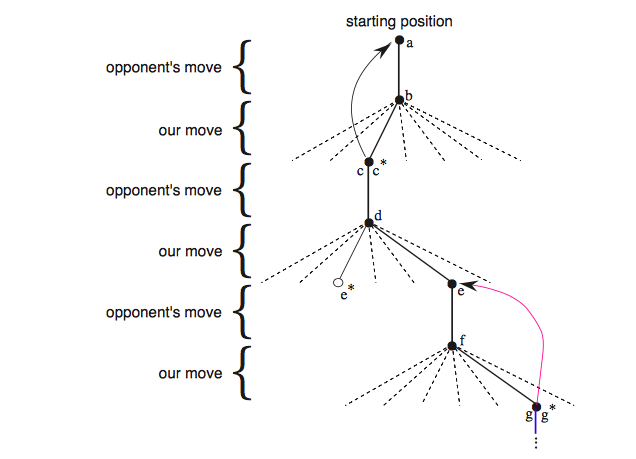
\includegraphics [scale=0.60] {game_tree.png}
\end{center}

Przypuśćmy dalej, że z każdym stanem końcowym gry (liściem) może powiązać liczbę wygranych punktów. W przypadku gier takich jak kółko i krzyżyk, może to być jedna z trzech wartości ${-1, 0, 1}$  odpowiadająca przegranej, remisowi i wygranej odpowiednio.  Możemy jednak wyjść poza ten schemat i rozważać dla stanów końcowych wiele innych wartości.  Ważne jest to, że celem gracza jest maksymalizacja zdobytych punktów. Warto jeszcze zaznaczyć, że punkty przypisane do liście są różne dla rywalizujących ze sobą graczy. W naszym przypadku gry w kółko i krzyżyk, suma punktów zdobytych przez jednego rywala, będzie równa sumie punktów zdobytych przez drugiego rywala, ale z przeciwnym znakiem.  W ogólnym. przypadku jednak tak nie musi być. \\

 Można by naiwnie przypuszczać, że najlepszą strategią będzie wybranie takiego ruchu, który ,,otworzy'' nam ścieżkę do liści z największą możliwą ilością punktów. Zobaczymy na poniższym przykładzie wziętym ze strony \cite{Game}, że taka strategia nie jest optymalna. Wyobraźmy sobie dwie konkurujące ze sobą firmy, które rozważają poniesienie wydatków na promocję oferowanego przez siebie produktu. Firma 1 pierwsza będzie podejmować decyzję, czy inwestować w reklamę, czy też nie.  Ta decyzja odpowiada pierwszemu rozgałęzieniu na poniższym drzewie. Kolejna decyzja  należy do firmy drugiej - inwestować w reklamę lub nie. W sumie mamy cztery możliwe sytuacje (cztery różne rozgrywki) i odpowiadające im punkty (można je interpretować np. jako zysk). \\

\begin{center}
	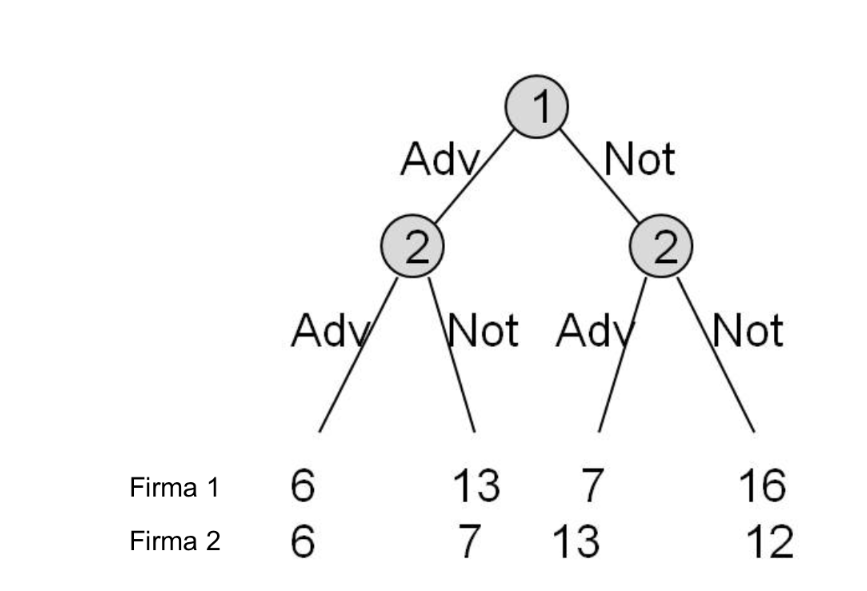
\includegraphics [scale=0.30] {advertise.png}
\end{center}
 
 Jeżeli obie firmy nie zdecydują się nie inwestować w reklamę, to firma 1 zdobędzie 16 punktów, a firma 2 - 12 punktów. Przyjmijmy, że koszt reklamy to 8 punktów. Jeżeli jedna firma zdecyduje się na reklamę, a druga nie, to firma reklamująca uzyska 13 punktów, a firma która nie reklamowała swojego produktu 7 punktów (firma reklamująca się zdobywa 21 punktów z 28 dostępnych, ale ponosi 8 punktowy koszt reklamy).  Natomiast jeżeli obie firmy zdecydują się na reklamę, to podzielą między siebie rynek po równo, ale ponieważ każda z nich poniesie koszt 8 punktów, to finalnie każda zarobi po 6 punktów ($(28 - 16)/2$).\\
 
 Załóżmy, że jesteśmy prezesem firmy 1 i chcemy podjąć decyzję o tym, czy inwestować w reklamę czy też nie. Załóżmy dalej, że drzewo przedstawiające możliwe wyniki tej gry jest znane wszystkim zainteresowanym stronom. Wówczas logicznym będzie następujące rozumowanie. Jeżeli firma 1 zdecyduje się na reklamę, to firma 2 chcąc maksymalizować liczbę zdobytych punktów nie będzie się reklamować. Wówczas firma 1 zdobędzie 13, a firma 2  - 7 punktów.  Z drugiej strony, jeżeli firma 1 zdecyduje się nie reklamować, to firma 2 znowu maksymalizując swoją wygraną zainwestuje w reklamę i końcowy wynik będzie 7 i 13 punktów dla firmy 1 i firmy 2 odpowiednio.  Ponieważ pierwszy scenariusz jest korzystniejszy, to firma 1 decyduje się na inwestycję w reklamę. \\
 
 Z powyższego, bardzo prostego rozumowania, wynika kilka wniosków. Po pierwsze, przy założeniu, że oponent (firma 2 w tym przypadku) racjonalnie usiłuję maksymalizować liczbę zdobytych punktów, to wybór ,,otwierający'' drogę do liści z największą liczbą punktów nie musi być wyborem optymalnym. Firma 1 mogłaby zdecydować nie reklamować się, bo wówczas jej potencjalna wygrana, to 7 lub 16 punktów versus 6 i 13 przy reklamowaniu się. Taka strategia byłaby słuszna gdyby firma 2 losowo podejmowała decyzje, ale nie jeżeli firma  2 ma racjonalnych decydentów. Druga obserwacja, często podnoszona w teorii gier, że najlepsze rozwiązanie dla obydwu firm - nie reklamować swoich produktów  - jest rozwiązaniem niemożliwym lub przynajmniej nie stablinym. Teoretycznie prezesi firm mogli się zmówić, że nie będą inwestować w reklamę.  Ale w takiej sytuacji, o ile firma 1 rzeczywiście zdecyduje nie reklamować się, to firma 2, chcąc maksymalizować swoje punkty, powinna zdecydować się na reklamę i tym samym złamać umowę. Stąd wspomniana wyżej niestabilność.\\
 
Na powyższym przykładzie można też zrozumieć w jaki sposób wybrać optymalny ruch. Załóżmy, że reprezentujmy firmę 1. Do nas należy otwierający ruch. Racjonalnie będzie założyć, że po naszym ruchu firma 2 wykona ruch, który pozwoli w ostatecznym rachunku na maksymalizację jej wygranej, co przy stałej puli możliwych do wygrania punktów, będzie tożsame z takim ruchem, który zminimalizuje naszą wygraną. Zatem należy wybrać taki ruch, który maksymalizuje minimum z naszych wygranych do jakich może doprowadzić firma 2 kolejnym ruchem.  To rozumowanie naturalnie przekłada się na gry, których drzewa mają więcej pokoleń. W każdym przypadku konieczne jest przejście wszystkich węzłów drzewa idąc od liśc (tutaj wiem jakie są wygrane) biorąc pod uwagę dla każdego pokolenia czy jest nasz ruch, czyli ruch, czy też ruch naszego oponenta, który ma na celu minimalizowanie naszej wygranej. Przedstawiając powyższe rozumowanie w punktach dochodzimy do algorytmu minimax, który dla każdego węzła zwraca wygraną wartość gracza . \\

\begin{enumerate}
	\item{Jeżeli to jest ruch końcowy, to zwróć wartość wygranej i skończ}
	\item{Jeżeli ruch należy do nas, a nie do oponenta to:}
	\begin{enumerate}
		\item{ustawa wartość$=-\infty$}
		\item{Dla każdego możliwego dostępnego ruchu: }
		\item{wartość = max(wartość,  wartość algorytmu minimax na poddrzewie, którego korzeniem jest rozpatrywany ruch oponenta}
		\item{zwróć wartość}
	\end{enumerate}
		\item{Jeżeli ruch należy do oponenta to:}
	\begin{enumerate}
		\item{ustawa wartość$=+\infty$}
		\item{Dla każdego możliwego dostępnego ruchu: }
		\item{wartość = min(wartość,  wartość algorytmu minimax na poddrzewie, którego korzeniem jest rozpatrywany ruch dla nas}
		\item{zwróć wartość}
	\end{enumerate}
\end{enumerate}


Okazuje się, że jeżeli gracze stosują się do powyższego algorytmu, to znaczy wybierają ruchy, które zapewnią im największą wygraną wyliczoną według powyższego algorytmu, to takie strategie będą w równowadze Nash'a. Mówiąc obrazowo są  to najlepsza strategie, w tym sensie, że żadnemu z graczy nie opłaca się ich zmieniać. Jeżeli wiem, że mój oponent będzie grał zgodnie z algorytmem minimax, to moją najlepszą strategią będzie robić to samo. Jeżeli mój oponent będzie grał inną strategią, to być może istnieje lepsza odpowiedź na jego strategie niż minimax.  Jeżeli ja gram według algorytmu minimax, a mój oponent nie, to gra strategią suboptymalną. 

\section{Przycinanie $\alpha$ - $\beta$}
Podstawowym problemem w zastosowaniach algorytmu minimax jest ilość niezbędnych operacji przy dużych drzewach reprezentujących gry.  Dla gry w kółko i krzyżyk, górnym ograniczeniem ilości możliwych gier (liści na drzewie gry) jest $9! = 362880$. W rzeczywistości ilość możliwych partii ogranicza się do kilku tysięcy, ale i tak przeliczenie wszystkich węzłów takiego drzewa na współczesnym komputerze średniej klasy zajmuje kilka sekund (przynajmniej przy amatorskiej implementacji autora niniejszej pracy). Jeżeli pomyśleć o grach takich jak szachy, w których ilość możliwych ruchów i łączna ilość ruchów w grze jest ogromna, to jasnym się staje, że algorytm minimax ma poważne ograniczenia.  \\

W praktyce, żeby ograniczyć ilość wykonywanych operacji stosuje się tzw. przycinanie  $\alpha$ - $\beta$. Polega to na tym, że jeżeli wiemy, że sprawdzenie i porównanie wartości dla kolejnego ruch/węzła na drzewie gry nie zmieni wyboru gracza , to pomijamy takie obliczenie. Najlepiej zobaczyć to na prostym przykładzie. 
\begin{center}
	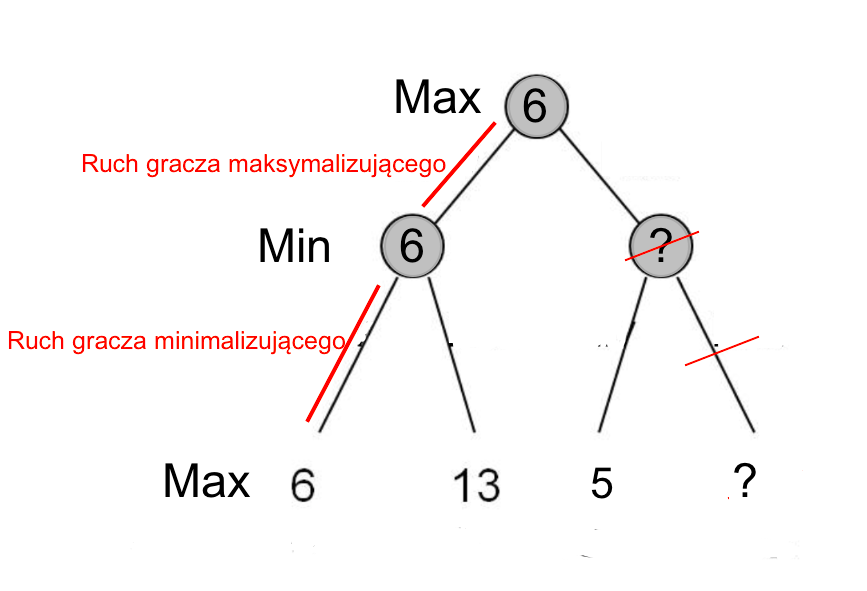
\includegraphics [scale=0.3] {advertise2.png}
\end{center}
Spójrzmy raz jeszcze na poprzedni przykład, ale nieco zmieniony. Jesteśmy graczem rozpoczynającym grę i chcemy wybrać optymalny ruch za pomocą algorytmu minimax. Minimax jest algorytmem rekurencyjnym; żeby policzyć wartości wygranej dla każdego z możliwych ruchów, trzeba "wywołać" minimax dla gracza minimalizującego na odpowiednich poddrzewach. To z kolei sprowadza się do porównywania wszystkich wartości liści, czyli ostatecznej wygranej w grze i następnie sukcesywnego podążania w górę drzewa.  Idąc od lewego dolnego liścia widzimy, że gracz minimalizujący będzie miał wygraną 6, bo  na pewno nie wybierze liścia z wartością 13 (minimalizuje naszą wygraną). Czyli jeżeli wybierzemy ruch "w lewo", to nasza wygrana, to będzie 6. Jeżeli zaczniemy kalkulować wygraną w przypadku ruch "w prawo", to widzimy, że nasz oponent wybierze 5 albo jeszcze mniej gdyby w skrajnym prawym liściu była mniejsza wartość. Ale ten fakt jest dla nas, dla gracza maksymalizującego, już bez żadnego znaczenia. Decydując się na ruch "w lewo" wygramy 6, a decydując się na ruch "w prawo" wygramy co najwyżej 5. Możemy zatem w ogóle nie sprawdzać jaka jest wartość prawego skrajnego liścia i nie wyliczać wartości wygranej gdybyśmy wykonali ruch "w prawo". Tym sposobem zaoszczędziliśmy trochę obliczeń. 
\begin{flushleft}
	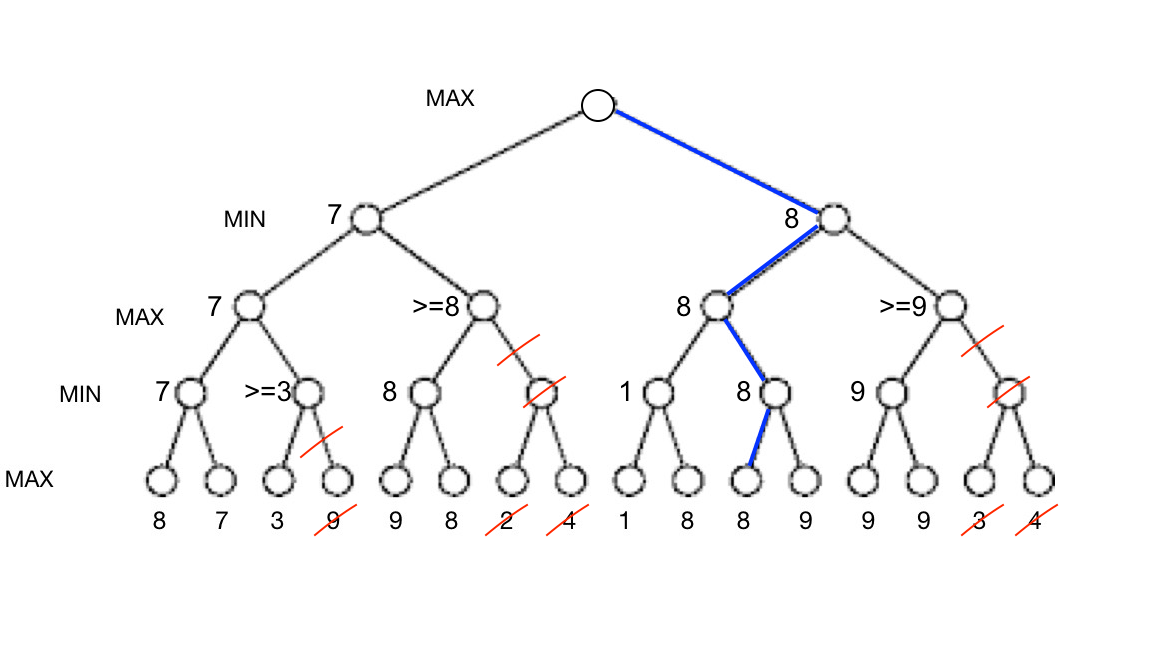
\includegraphics [scale=0.45] {big_tree2.png}
\end{flushleft}
Załóżmy, że mamy do czynienia z takim drzewem gry jak na rysunku. Ostatni wiersz przedstawia możliwe wygrane gracza maksymalizującego, rozpoczynającego grę. Na rysunku zaznaczono węzły i całe podrzewa, których gracz maksymalizujący nie potrzebuje rozpatrywać. Po lewej stronie węzłów zapisana jest maksymalna możliwa wygrana gracza maksymalizującego o ile gra znajdzie się w tym weźle (czyli wartość jaką zwraca algorytm minimax). Pogrubioną linią widać optymalną ścieżkę gry, która kończy się zdobyciem 8 punktów. Dla zwięzłości pracy nie opisuję całego toku rozumowania. Przykład ten wzięty jest z 6 wykładu profesora Winstona z \cite{MIT_AI}.\\

Jak widać, w niektórych przypadkach udaje się sporo zaoszczędzić w ilości obliczeń.  Warto jeszcze wyjaśnić skąd $\alpha - \beta$ w nazwie. Zaczynając przeszukiwanie drzewa ustawiamy parametry $\alpha$ i $\beta$ na $+\infty$ i $-\infty$ odpowiednio, i interpretujemy je jako najgorszy możliwy wynik gracza minimalizującego ($+\infty$) i  najgorszy możliwy wynik gracza maksymalizującego ($-\infty$). Przechodząc rekurencyjnie przez drzewo sprawdzamy aktualizujemy wartości $\alpha$ i $\beta$ i jeżeli dla danego poddrzewa  nie możemy poprawić wyniku  $\alpha$ lub  $\beta$ (w zależności czy dla tego poddrzewa pierwszy ruch należy do gracza minimalizującego lub maksymalizującego), to nie przeszukujemy dalej tego poddrzewa.


\section{Funkcja wartości}
Nietrudno wyobrazić sobie, że dla gier z olbrzymimi drzewami gry, przycinanie $\alpha$ - $\beta$ pomoże nam zejść o o kilka pokoleń w dół drzewa, ale i tak nawet najszybszy komputer nie jest w stanie przeszukać całego drzewa w takiej grze jak szachy. W związku z tym,  algorytmy grające w takie gry wykorzystują \textbf{funkcję wartości}. Jest to funkcja zwracająca pewną wartość (scoring) dla każdego stanu gry. Czym wyższa wartość, tym bardziej korzystna sytuacja dla gracza. \\

Algorytm grający będzie z reguły miał zaszyty parametr, który każe przerwać przeszukiwanie drzewa na danym poziomie lub po przekroczeniu określonej ilości czasu. Następnie ze wszystkich możliwych ruchów (liści z przeszukanego poddrzewa do momentu zastopowania algorytmu) wybierany jest ten dla którego, funkcja wartości przyjmuje maksymalną wartość. Dla szachów funkcja wartości może np. zliczać ilość punktów (każda figura ma przypisaną liczbę punktów - pionek 1, koń 5 , wieża 8 itd)  gracza i oponenta figur będących na planszy. 


\section{Implementacja}
Szczegóły dotyczące implemetacji, jak również kod można znaleźć w \textbf{DODATEK B}. W tej sekcji chciałbym ograniczyć się do kilku spostrzeżeń związanych z implementacją algorytmu minimax z przycinaniem $\alpha - \beta$.\\

Liczyłem na to, że zastosowanie przycinania zmniejszy czas wykonania algorytmu na początku gry, w pierwszych dwóch ruchach,  kiedy konieczne jest przeszukanie największych drzew. Od trzeciego ruchu, wykonanie algorytmu jest rzędu $0.1$ sekundy, więc optymalizacje przestają mieć znaczenie.  Niestety zastosowanie przycinania $\alpha - \beta$ nie poprawiło w widoczny sposób szybkości działania algorytmu. Żeby ograniczyć czas oczekiwania na odpowiedź komputera dodałem instrukcję, powodującą, że jeżeli algorytm zaczyna grę, to zawsze wybiera środkowe pole.\\

Nie udało mi się też zaimplementować algorytmu z ograniczeniem głębokości przeszukiwania drzewa i wykorzystującego funkcję wartości. Banalne funkcje wartości typu sprawdzenie,  czy mam dwa krzyżyki(kółka) w linii nie dawały dobrych rezultatów. Tak skalibrowany algorytm popełniał oczywiste błędy i łatwo z nim było wygrać.  Natomiast uwzględnienie większej ilości niuansów, w zasadzie prowadziło mnie  do napisania reguły jak grać w kółko i krzyżyk. Wówczas minimax przestaje być potrzebny i można się ograniczyć do do policzenia funkcji wartości dla możliwych ruchów i wybrania tego z największą wartością. Niestety nie udało mi się znaleźć ,,złotego środka'' i w końcowej implementacji nie korzystam z funkcji wartości. \\

Algorytm minimax jest graczem optymalnym, nie można grać lepiej od algorytmu minimax. W szczególności, można co najwyżej zremisować. W dalszej części pracy algorytm minimax będzie obok gracza losowego (takiego co losuje z jednostajnym prawdopodobieństwem kolejny ruch z puli możliwych) punktem odniesienie skuteczności algorytmu grającego w kółko i krzyżyk. Skuteczne algorytmy powinny często remisować i rzadko przegrywać z minimax, oraz często wygrywać i rzadko remistować z minimax. Poniżej przedstawiam wyniki partii 100 gier rozegranych pomiędzy graczem stosującym minimax oraz graczem losowym  oraz 100 gier rozegranych pomiędzy dwoma graczami stosującymi algorytm minimax.\\ 

\begin{flushleft}
	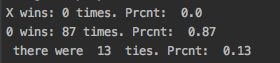
\includegraphics [scale=0.6] {random_minimax.png}
\end{flushleft}

Gracz stosujący minimax nie przegrał ani razu, za to zremisował z graczem losowym 13 razy na 100 gier.

\begin{flushleft}
	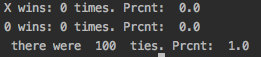
\includegraphics [scale=0.6] {minimax_minimax.png}
\end{flushleft}
Dwóch graczy stosujących minimax zawsze będą ze sobą remisować. 

\chapter{Q-learning}\label{r:Tablica}

\section{Procesy decyzyjne Markowa}
W rozdziale pierwszym gry były reprezentowane (a w zasadzie wszystkie możliwe rozgrywki) za pomocą drzew, gdzie węzły należały do możliwych stanów gry, a krawędź pomiędzy dwoma węzłami oznaczała przejście na skutek ruchu jednego z graczy do kolejnego stanu. W tym rozdziale skoncentruję się na innym modelu, a mianowicie na procesach decyzyjnych Markowa.  Przed formalnymi definicjami kilka chciałbym przedstawić heurystyczny opis modelu, posiłkując się rysunkiem wziętym z \cite{RL}.\\

\begin{flushleft}
	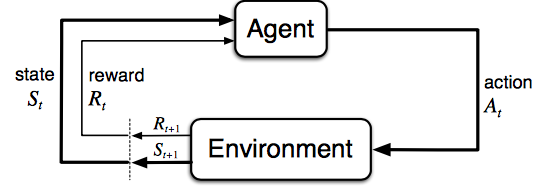
\includegraphics [scale=0.6] {agent_env.png}
\end{flushleft}

Załóżmy, że mamy agenta (gracza w naszym przypadku), który jest w interakcji z pewnym systemem (\textit{environment} na rysunku). Agent znajduje się w pewnym stanie $s$, w dyskretnym czasie $t$ i ma do wyboru podjęcie jednej z dostępnych akcji $a\in\mathcal{A}$. Na skutek podjęcia akcji $a$ system odpowie przejściem do nowego stanu $s'$ oraz nagrodą $r$ (z ang. \textit{reward}) w czasie $t+1$.  Nie jest przy tym powiedziane, że dla konkretnej pary $(s,a)$ system zawsze przejdzie do tego samego stanu $s'$. System może wybierać swoją odpowiedź losowo. Podobnie przy przejściu ze stanu $s$ do $s'$ system może losowo zwracać różne nagrody $r$.  Natomiast ta losowość musi zależeć tylko i wyłącznie od pary $(s,a)$ i nie może w żaden sposób zależeć od poprzednich stanów w jakich system się znajdował. Na tym polega istota ,,markowości", że historia nie ma znaczenia. W tym miejscu chciałbym poczynić jeszcze jedno założenie, że zbiór możliwych stanów systemu jest skończony. To założenie nie jest konieczne w ogólnej teorii, ale pozwala na daleko idące uproszczenia, z których skrzętnie korzystam w tej, jakby nie było, ilustratywnej pracy. Interakcja agenta z systemem przez kilka kolejnych kroków począwszy od $t=0$ można przedstawić za pomocą takiej trajektorii:
$$s_{o}, a_{0}, r_{1}, s_{1}, a_{1}, r_{2}, s_{2}, a_{2}, r_{3}, s_{3},...$$

Formalizując powyższe rozważmy czwórkę postaci $<\mathcal{S},\mathcal{A},\mathcal{R},p>$ gdzie:
\begin{enumerate}
 	\item{$\mathcal{S}$ jest skończonym zbiorem możliwych stanów systemu}
	\item{$\mathcal{A}$ jest zbiorem możliwych akcji. Formalnie $\mathcal{A}$ jest kolekcją zbiorów $\mathcal{A}_{s}$ indeksowaną stanami $s\in\mathcal{S}$. Chodzi o to, że dla różnych stanów systemy dostępne są różne akcje.  Dla uproszczenie będę jednak pomijali ten niuans notacyjny i w dalszej części mówił o możliwych akcjach $\mathcal{A}$  pamiętając, że ten zbiór może być ograniczony konkretnym stanem.}
	\item{$\mathcal{R}\subseteq\mathbf{R}$ jest zbiorem wartości nagród, jakie agent może otrzymać}
	\item{$p:\mathcal{S}\times\mathcal{A}\times\mathcal{R}\times\mathcal{S}\rightarrow [0,1]$ jest funkcją determinującą dynamikę procesu decyzyjnego Markowa. Dla każdej pary stanu i wyboru 		akcji w czasie $t$ funkcja $p$ określa rozkład prawdopodobieństwa na $\mathcal{R}\times\mathcal{S}$ w czasie $t+1$:  $$p(s, a, s', r) = \mathbf{P}(S_{t+1}=s', R_{t+1}=r | S_{t}=s, A_{t}=a )$$}
\end{enumerate}

Opisany model z powodzeniem można stosować do opisu gry w kółko i krzyżyk (jak również innych turowych gier). Przestrzeń stanów $\mathcal{S}$ w tym wypadku to będą wszystkie możliwe stany gry. Akcje $\mathcal{A}$ to będą wszystkie możliwe ruchy do wykonania przy danym stanie gry. Agentem jest gracz - algorytm, którego staram się nauczyć grać w kółko i krzyży. Systemem natomiast jest drugi gracz - może to być gracz losowy lub gracz stosujący algorytm minimax. Pozostaje jeszcze określenie nagród $\mathcal{R}$. Wybór jest poniekąd arbitralny, ale ponieważ celem będzie maksymalizowanie wartości oczekiwanej nagród, to należy pamiętać, że algorytm wyuczy się osiągania średnio wysokich nagród, a nie wygrywanie. \\

Zanim przejdę do opisu algorytmu potrzebne będzie jeszcze kilka pojęć. \textbf{Strategią} nazwiemy dowolne mapowanie 
$$\pi : \mathcal{S}\rightarrow\mathbf{P}_{\mathcal{A}} \text{, gdzie } \forall_{s\in\mathcal{S}} \text{ } \pi(s) \text {  jest rozkładem prawdopodobieństwa na } \mathcal{A}$$ 
Celem gracza będzie dążenie do takiej strategii, która maksymalizuje wartość nagród otrzymanych podczas gry.  W procesach decyzyjnych Markowa często stosuje się dyskontowanie przyszłych nagród wybranym czynnikiem $\gamma\leq1$ Wynika to z dwóch powodów. Po pierwsze w zastosowaniach często przyszłe nagrody mają rzeczywiście niższą wartość niż obecnie (jak w matematyce finansowej) a po drugie, interakcja agenta z system może nie być ograniczona ilością ruchów, a wtedy suma przyszłych nagród niezależnie od wyboru strategii $\pi$ może być nieskończona, co uniemożliwia wybranie optymalnej strategii. Jeżeli natomiast maksymalna nagroda jest ograniczona, powiedźmy liczbą $M$, oraz $\gamma<1$, to suma nagród jest z góry ograniczona przez
$$M+\gamma M +\gamma^{2}M+\gamma^{3}M+...  = \frac{M}{1-\gamma}$$
Dla uproszczenia zapisu wprowadźmy oznaczenie na sumę przyszłych zdyskontowanych nagród:
$$G_{t} \stackrel{\text{def}}{=} R_{t} + \gamma R_{t+1} + \gamma^{2}R_{t+2} +...$$

Wartością stanu $s$ przy strategii $\pi$ jest z definicji 
$$v_{\pi}(s)\stackrel{\text{def}}{=} \mathbb{E}_{\pi}(G_{t}| S_{t} = s) $$
Jest to wartość oczekiwana sumy dyskontowanych przyszłych nagród pod warunkiem, że stosujemy strategię $\pi$ począwszy od czasu $t$. w którym to czasie system znajdował się w stanie $s$. 
Podobnie zdefiniujmy jeszcze funkcję określającą wartość akcji $a$ podjętą w stanie $s$ jako zdyskontowaną wartość przyszłych nagród przy założeniu, że stosujemy strategię $\pi$, a w stanie $s$ wybierzemy akurat akcję $a$ (strategia $\pi$ zadaje rozkład prawdopodobieństwa na $\mathcal{A}$, i w tej definicji zakładamy, że akurat wylosowano akcję $a$):
$$q_{\pi}(a,s) \stackrel{\text{def}}{=} \mathbb{E}_{\pi}(G_{t}| S_{t} = s, a_{t} = a) $$

Co zatem oznacza znalezienie optymalnej strategii? Intuicyjnie jest to oczywiste. Chcemy mieć strategię, która będzie maksymalizować wartość oczekiwaną sumy przyszłych zdyskontowanych nagród. Formalnie $\pi_{1}\prec\pi_{2}$ jeżeli dla każdego $s\in\mathcal{S}$ zachodzi $$v_{\pi_{1}}(s)\leq v_{\pi_{1}}(s)$$
Powiemy, że $\pi_{*}$ jest optymalna, jeżeli dla każdej strategii $\pi$ zachodzi   $\pi\prec\pi_{*}$ Nietrudno przy tym zauważyć, że jeżeli $\pi_{*}$ jest optymalną strategią, to spełnione będą równiania:
$$v_{\pi_{*}}(s) =\max_{\pi} v_{\pi}(s)$$ $$q_{\pi_{*}}(a,s) = \max_{\pi} q_{\pi}(a,s)$$

Dopiero teraz przechodzimy do pytania jak znaleźć optymalną strategię? Dzięki temu, że zbiory $\mathcal{S}, \mathcal{A}, \mathcal{R}$ są skończone, to znajomość funkcji $p$ daje nam  ,,pełną wiedzę" o systemie. W szczególności można dokładnie wyliczyć optymalną strategię, bazując na tzw. równiach Bellman'a, które wiążą $v_{\pi}(s)$ z kolejnym stanem systemu $v_{\pi}(s')$
$$v_{\pi}(s) = \sum_{a}\pi(a|s)\sum_{s',r}p(s,a,s',r)[\gamma +\gamma v_{\pi}(s')] $$

Rozsupłanie powyższej ,,rekurencji'' i znalezienie optymalnej strategii  można  sprowadzić  do rozwiązania $|\mathcal{S}|$  równań liniowych i policzenia wartości $v_{\pi}(s)$  dla każdego stanu $s$ dla arbitralnie wybranej deterministycznej (nie losowej )strategii $\pi$. Następnie można ,,poprawiać'' $\pi$ poprzez sprawdzanie, czy dla poszczególnych stanów $s$ i $a$ (takich, że $\pi(s)\neq a$ )będzie $q_{\pi}(s,a)\geq v_{\pi}(s)$. Jeżeli znajdziemy ,,lepszą'' akcję $a$  dla stanu $s$ aniżeli $\pi(s)$, to mamy poprawioną strategię 
$$\pi'(s) =
	\begin{cases}
		a\text{ ,  }s=a,\\			
		\pi(s)\text{ , } s\neq a\\
	\end{cases}
$$
 Okazuje się, że takie poprawianie strategii $\pi\rightarrow\pi'\rightarrow\pi''\rightarrow ...$ prowadzi do optymalnej strategii $\pi_{*}$. Takie podejście w \cite{RL} nazywane jest programowaniem dynamicznym (z ang. \textit{dynamic programming}). Jest to skuteczne podejście jeżeli mamy pełną wiedzę o funkcji $p$ Najczęściej tak jest, jeżeli modeluje się jakieś rzeczywisty system za pomocą procesu decyzyjnego Markowa.\\

Nas jednak bardziej interesuje sytuacja, w której nie znamy funkcji $p$ i będziemy chcieli stworzyć algorytm, które znajduje optymalną strategię doświadczalnie, czyli algorytm, który będzie uczył się systemu, bez uprzednich założeń odnośnie funkcji $p$. Najczęściej zaczyna się od losowej strategii i z każdym cyklem interakcji z systemem (albo po $n$ cyklach) dostosowujemy strategię na podstawie dotychczasowych obserwacji. Ponieważ $v_{\pi}(s)$ jest definiowana jako wartość oczekiwana, to naturalnym odruchem może być wyliczanie przyszłych nagród startując ze stanu $s$ i podążając za strategią $\pi$ w wielu epizodach iterakcji agenta z system, a następnie uśrednienia otrzymanych wartości. Takie podejście, typowo w stylu monte-carlo, ma poważną wadę w przypadku systemów z dużą ilością stanów, bo potrzeba czasami nierealistycznie dużej próbki danych (epizodów), żeby sensownie policzyć  $v_{\pi}(s)$. \\
 
 Metodą, poniekąd łączącą, programowanie dynamiczne z metodami w stylu monte carlo nie wymagających znajomości funkcji $p$ są metody Q-learning (albo ogólnej z ang. \textit{temporal difference}).  Idea tych metod sprowadza się do tego, że możemy w każdy kroku, po każdej interakcji agenta z systemem, poprawiać stosowaną przez niego strategię $\pi$ zgodnie ze wzorem
\begin{equation}
   v_{\pi}(s_{t}) := v_{\pi}(s_{t}) +\alpha [R_{t+1} + \gamma v_{\pi}(s_{t+1}) - v_{\pi}(s_{t+1})]
 \end{equation}
 W tym wypadku nie potrzebujemy czekać do końca epizodu (np. do końca gry), a najlepiej wielokrotnie, żeby zaktualizować $v_{\pi}(s_{t})$ jak w metodach monte carlo. Możemy bazować tylko na otrzymanej nagrodzie i estymacji $v_{\pi}(s_{t+1})$ dla kolejnego stanu. Tutaj $\alpha$ jest hiperparametrem algorytmu, często nazywany z angielskiego \textit{learning rate}. 
 
\section{Opis algorytmu}
Strategię zdefiniowaliśmy jako mapowanie, które każdemu stanowi $s\in\mathcal{S}$ przypisuje rozkład prawdopodobieństwa $\mathbf{P}_{s}$ na przestrzeni stanów $\mathcal{A}$. Teraz jednak chcemy przejść od ogólnej teorii do konkretnego algorytmu grającego w kółko i krzyżyk i w tym celu dokonamy kilku uproszczeń. W szczególności ograniczmy się do strategii nie losowych, tzn, do mapowania
$$\pi : \mathcal{S}\rightarrow\mathcal{A}$$
Jest to szczególny przypadek opisanej w poprzedniej sekcji teorii, gdzie rozważamy wyłącznie atomowe rozkłady prawdopodobieństwa na $\mathcal{A}$. Mając danych stan $s\in\mathcal{S}$ chcemy znać optymalny ruch $\pi(s)\in\mathcal{A}$.  Przy takim uproszczeniu:
	$$\pi_{*}(s) = \argmax_{a\in\mathcal{A}} q(a,s)$$
		oraz
	$$v_{\pi_{*}}(s)=\max_{a\in\mathcal{A}} q(a,s)$$
Optymalna strategia, przy założeniu że znaleźliśmy się w stanie $s$ będzie maksymalizować oczekiwaną nagród wartość $q(a,s)$. Teraz chcielibyśmy włożyć te uproszczenia do (2.1) i na tej podstawie wypracować algorytm nadający się do implementacji. Na początek możemy położyć dla każdego stanu $s\in\mathcal{S}$ i dla każdej akcji $a$, $q(a,s) = 0$.  Dalej załóżmy, że wykonujemy pierwszy cykl interakcji  z systemem. W przypadku gry w kółko i krzyżyk nasz oponent wykonał ruch i gra jest w stanie $s$. Teraz kolej na agenta, który dąży do tego, żeby nauczyć się optymalnej strategii. Zgodnie z (2.2) agent powinien rozważyć wszystkie możliwe ruchy $a$ i wybrać ten, który maksymalizuje $q(a, s)$. Jeżeli jest więcej niż jedno takie $a$, to gracz wybiera je losowo. W każdym razie gracz wybiera  $\tilde{a}$, które maksymalizuje wszytskie $q(a,s)$. System znowu odpowiada na ruch $\tilde{a}$  i przechodzi do stanu $\tilde{s}$ i zwraca nagrodę $R$. Teraz podstawiając $q(\tilde{a},s)$ za $v_{\pi}(s)$ do (2.1) otrzymujemy przypis jak je  zmienić:\\
\begin{equation}
\label{q}
	q(\tilde{a},s) := q(\tilde{a},s) +\alpha[R + \gamma\cdot\max_{a\in\mathcal{A}}q(a,\tilde{s})]
\end{equation}
Możemy zainicjować wszystkie $q(a,s):=0$, a następnie podczas wielokrotnie rozgrywanych gier z systemem aktualizować te wartości po każdym ruchu zgodnie z (\ref{q}). Okazuje się, że takie aktualizacje, albo poprawianie wartości $q(a,s)$ po każdym ruchu, zapewni zbieżność do rzeczywistych wartości  $q(a,s)$. Następnie stosując (2.1) otrzymujemy optymalną startegię gry w kółko o krzyżyk.

\section{Implementacja}

Z poprzedniej sekcji wynika, że powinniśmy zainicjować dla wszystkich możliwych stanów gry $s$ i możliwych ruchów $a$ wartości $q(a,s):=0$ i następnie aktualizować. Wypisanie do listy lub tabeli wszystkich możliwych kombinacji $(a,s)$ dla gry w kółko i krzyżyk jest oczywiście możliwe, aczkolwiek trochę kłopotliwe. Zauważmy również, że jeżeli po ruchu agenta  mamy jakiś rozkład kółek i krzyżyków na planszy, to nie ma znaczenia jaki był poprzedni stan i jaka akcja agenta doprowadziła do tegoż rozkładu kółek i krzyżyków. Innymi słowy, dla dowolnych dwóch par $(a', s')$ i $(a'', s'')$  jeżeli zarówno wybór akcji $a'$ w stanie $s'$ jaki i wybór $a''$ w stanie $s''$ prowadzi do takiego samego stanu gry $s$,  to $q(a', s') = q(a'', s'') = q_{s}$. Ta obserwacja skłania do przypisywaniu wartości $q_{s}$ do stanów gry po ruchu agenta. \\

W samej implementacji konieczne jest jeszcze ustalenia wartości nagród $\mathcal{R}$.  Wartości $q_{s}$ będą w procesie ,,uczenia''  algorytmu dążyć do oczekiwanej nagrody agenta, pod warunkiem, że swoim ruchem doprowadził do stanu $s$. Wybór jest poniekąd arbitralny, ale warto zauważyć, że w grze w ,,kółko i krzyżyk" remis jest dobrym wynikiem. Grając z graczem stosującym algorytm minimax można co najwyżej zremisować. Stąd potrzeba rozróżnienia przegranej, remisu i wygranej. Gdyby na przykład przypisać nagrodę 1 za wygraną, -1 za przegraną i 0 za każdy inny stan planszy, to algorytm grając z minimax uczyłby się tylko nie przegrywać. Nie byłby bowiem w stanie odróżnić wygranej od remisów. W tej implementacji przyjąłem wartości nagród równe: 
\begin{enumerate}
	\item{-1 w przypadku przegranej}
	\item{0.75 w przypadku remisu }
	\item{1 w przypadku wygranej}
	\item{0 dla każdego innego stanu gry}
\end{enumerate}

W implementacji wykorzystuję plik tekstowy, przechowujący wartości $q_{s}$, gdzie $q_{s}$, zgodnie z powyższą obserwacją jest równa wszystkim  $q(a',s')$, które prowadzą do stanu gry $s$ po podjęciu akcji $a'$ w stanie $s'$ przez agenta. Poniżej ilustruję kilka pozycji z tego pliku, już po przetrenowaniu algorytmu (około 20 000 gier rozegranych z graczem losowym) z omówieniem jego struktury.


\begin{flushleft}
	\includegraphics [scale=0.8] {QTable_ex.png}
\end{flushleft}

Pierwsze 9 cyfr rozdzielonych przecinkami przedstawia stan gry. Przy czym pierwsza cyfra opisuje pole w lewym górnym rogu planszy. Druga cyfra opisuje środkowe pole w górnym wierszu planszy. Trzecia cyfra pole w prawym górnym rogu. Kolejne trzy cyfry opisują środkowym rząd planszy idąc od lewej do prawej. Ostatnie 3 cyfry, opisują idąc od lewej do prawej dolny rząd planszy.  Cyfry 1 oznaczają ruchy systemu, czyli w tym wypadku człowieka, który gra z algorytmem. Cyfry 2 przedstawiają ruchy agenta, czyli grającego algorytmu. Cyfra 0 oznacza puste pole. Ostatnia liczba rzeczywista oznacza wartość  $q$ dla każdego ruchu agenta, który doprowadzi do stanu planszy reprezentowanego prze pierwsze 9 cyfr. 

Rozważmy pierwszy wiersz z powyżej ilustracji. Dla ustalenia uwagi załóżmy, że system gra ,,kółkiem", a agent ,,krzyżykiem". Ciąg $2, 0, 1, 2, 1, 2,  2, 1, 1.0$ Przedstawia od następujący stan gry po ruchu agenta.

\begin{flushleft}
	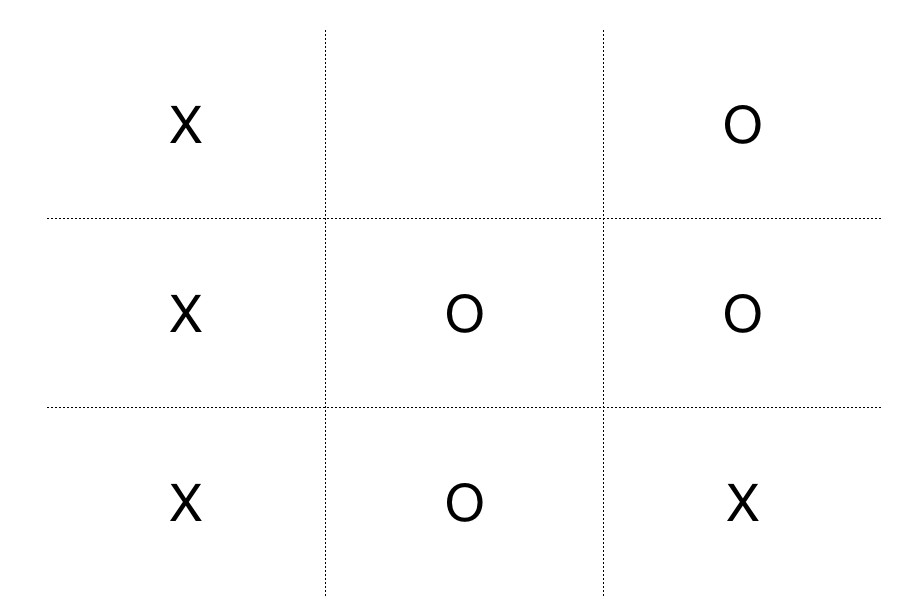
\includegraphics [scale=0.2] {ttt_1.png}
\end{flushleft}

To jest sytuacja w której agent wygrywa, stąd wartość $q$ dla tego stanu jest równa 1. \\
Kolejny wpis w tabeli, to ciąg $1, 2, 2, 2, 1, 1, 0, 1, 2, 0.75$. Pierwsze 9 cyfr przedstawiam następujący stan gry:

\begin{flushleft}
	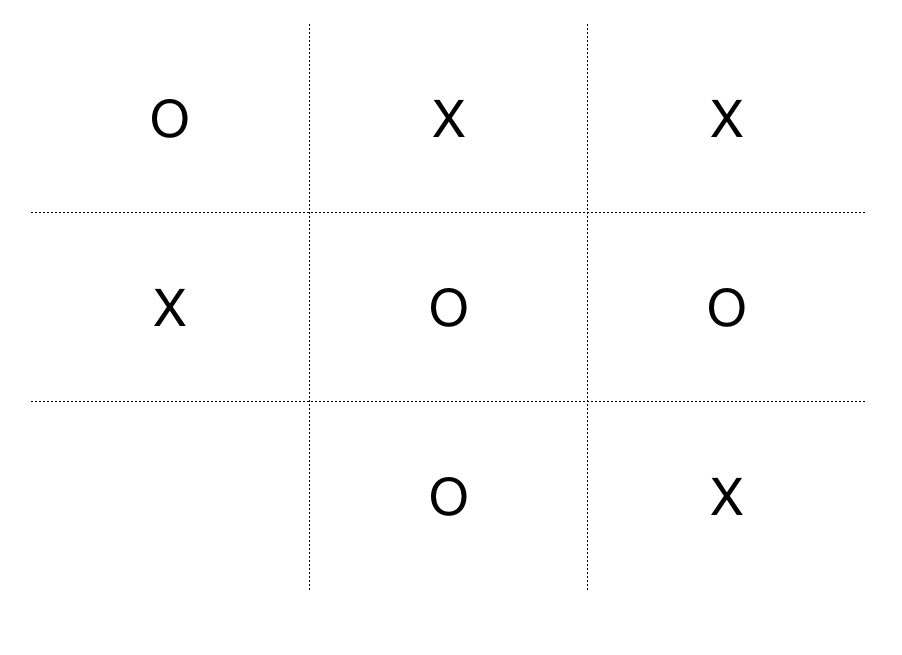
\includegraphics [scale=0.2] {ttt_2.png}
\end{flushleft}
Jak widać, niezależnie od ruchu gracza reprezentującego system (gracz posługujący się kółkiem), gra zakończy się remisem. Stąd wartość $q$ w tym przypadku jest równa $0.75$. \\

Kolejny przykład, to ciąg $2, 2, 1, 2,  2, 1, 1, 0, 0, -1$, jak łatwo zauważyć przedstawiam sytuację, w której  ruch należy do gracza systemowego (kółko lub cyfra 1) i gracz ten może z łatwością wygryać uzyskując trzy ,,kółka'' na prawej skrajnej kolumni. Stąd wartość $q$ w tym przypadku jest równa $-1$.
\begin{flushleft}
	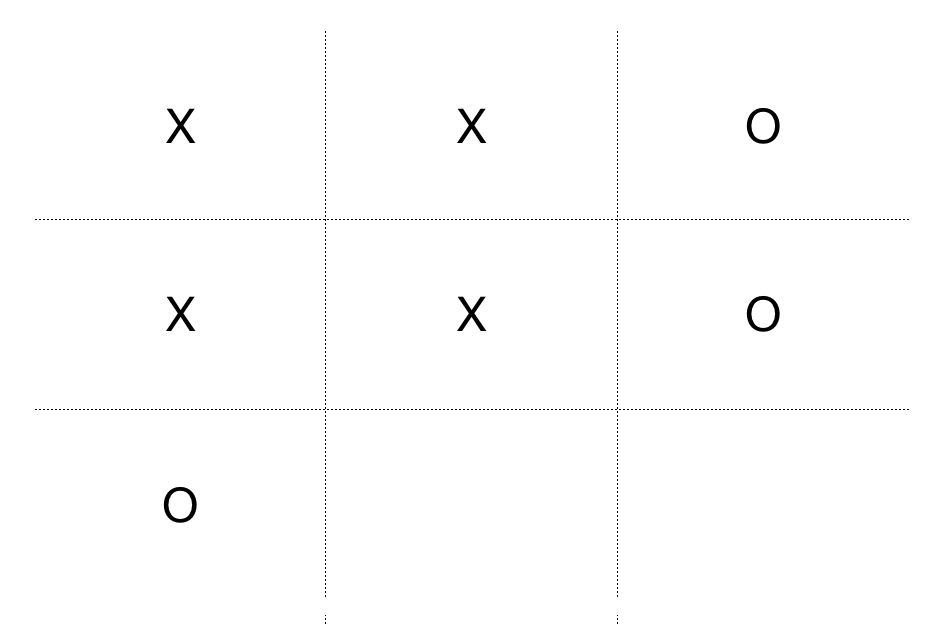
\includegraphics [scale=0.2] {ttt_3.png}
\end{flushleft}

Czwarty przykład odpowiadający ciągowi $2, 0, 0, 1, 2, 2, 0, 0, 0, 0.418681257165$  to gra w stanie jeszcze mało zaawansowanym, w którym obaj gracze mają szansę wygrać lub przegrać. W tym przypadku wyczuona wartość $q$ wynosi około $0.42$, co wskazywałoby, że jest to relatywnie korzystna sytuacja dla agenta grającego ,,krzyżykiem''.
\begin{flushleft}
	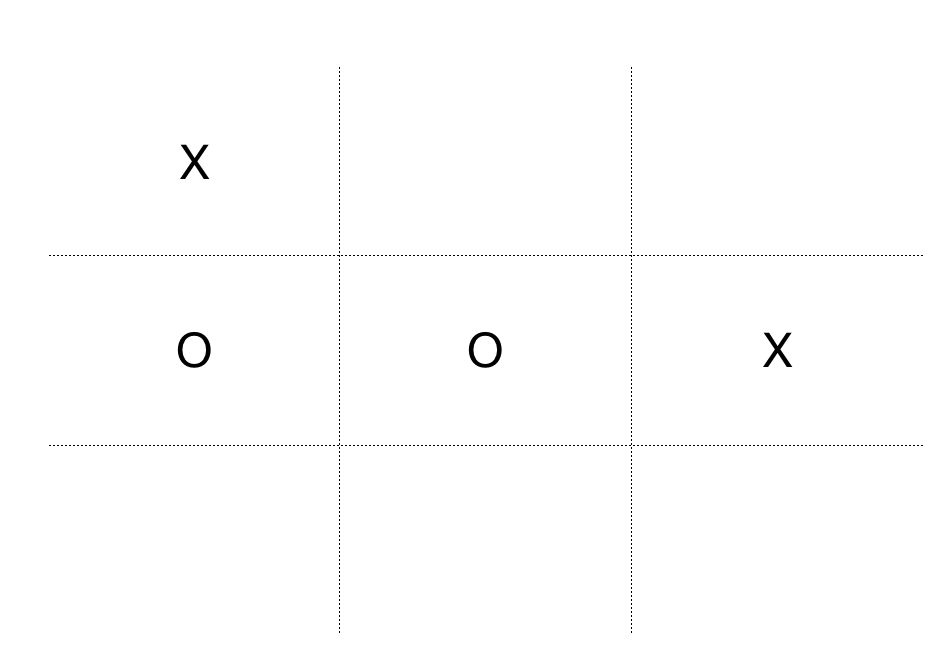
\includegraphics [scale=0.2] {ttt_4.png}
\end{flushleft}
Ostatni przykład, to ciąg $ 2, 0, 2, 2, 1, 0, 1, 1, 0, -0.0186631984604$ Wartość $q$ lekko ujemna wskazuje na neutralność tego stanu. Ten przykład jest ciekawy i pokazuje słabość algorytmu. System może w kolejnym ruchu wygrać grę. Pamiętajmy jednak, że algorytm uczył się grając z graczem losowym, który nie koniecznie wykorzysta możliwość wygrania i z tego stanu możliwe jest nadal zwycięstwo agenta (ale remis już nie). Przypuszczalnie dlatego wartość oczekiwana przyszłych nagród jest bliska zero. Gdyby uczyć algorytm poprzez grę tylko i wyłącznie z idealnym graczem, to najprawdopodobniej ten stan (po przetrenowaniu) miałby wartość bliższą $-1$.
\begin{flushleft}
	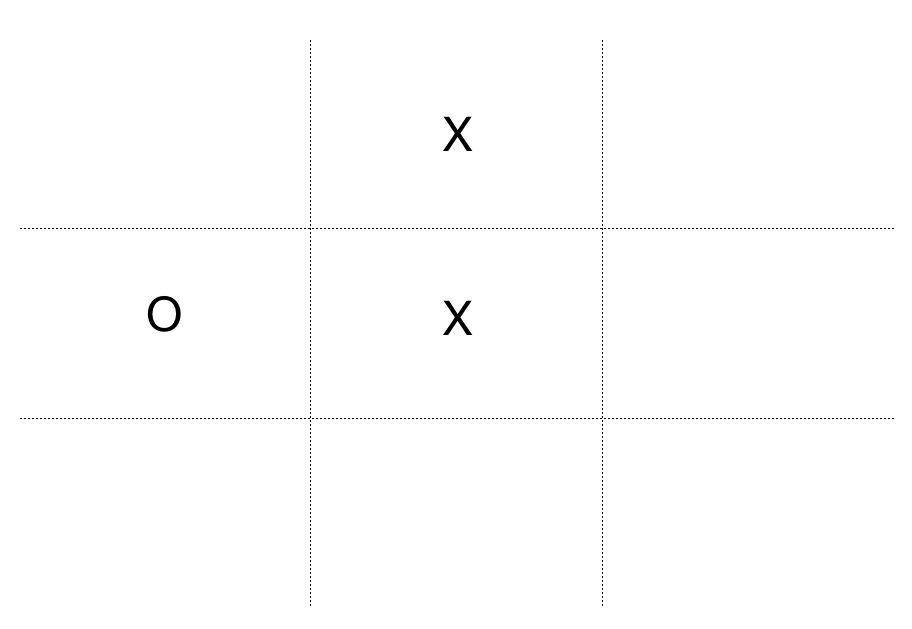
\includegraphics [scale=0.2] {ttt_5.png}
\end{flushleft}

Mając wszystkie niezbędne elementy możemy przejść do bezpośredniego zdefiniowania algorytmu:



Zaczynając od pustego zbioru wartości $q_{s}$, po 20 000 rozegranych grach z graczem losowym mamy zapisanych 


\begin{enumerate}
	\item{Inicjuj pusty zbiór z wartościami $q_{s}$}
	\item{Ustaw parametry $\alpha$ i $\gamma$ z przedziału $[0, 1]$}
	\item{Graj n razy z systemem w kółko i krzyzyk:}
	\begin{enumerate}
		\item{Jeżeli jest ruch agenta, a plansza jest w stanie $s-1$:}
		\begin{enumerate}
			\item{Dla każdego legalnego ruchu prowadzącego z $s-1$ do $s$  sprawdź wartość $q_{s}$ w zbiorze, a jeżeli nie ma takiego elementu w zbiorze to przyjmij $q_{s}=0$.}
			\item{Wybierz ten ruch $\tilde{s}$, dla którego $q_{\tilde{s}} =\max_{s} q_{s}$. Jeżeli jest kilka takich ruchów, to wybierz jeden losowo.}
			\item{Połóż $q_{s-1} = q_{s} + \alpha(R(\tilde{s}) + \gamma  q_{\tilde{s}} )$ }
			\item{Zapisz nową wartość $q_{s-1}$ w zbiorze. Jeżeli wartość już istniała w zbiorze, to nadpisz.}
		\end{enumerate}
	\end{enumerate}
\end{enumerate}

Popatrzmy teraz na wyniki uczenia. Zaczynam od pustego zbioru $q_{s}$ i rozgrywam po 100 partii z graczem losowym i z graczem stosującym minmax. Dodatkowo po każdej grze ,,opróżniam" zbiór $q_{s}$ tak żeby algorytm na razie niczego nie uczył się. Robię to po to, żeby mieć punkt odniesienia przy sprawdzaniu na ile dobrze algorytm nauczył się gry. W poniżyszych przykładach agent jest zawsze graczem korzystającym z ,,kółka", a system jest reprezentowany przez ,,krzyżyk". \\

W 100 grach rozegranych z graczem losowym otrzymałem wyniki jak poniżej:
\begin{flushleft}
	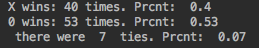
\includegraphics [scale=0.7]{Qtable_vs_Rnd_untrained.png}
\end{flushleft}
Jak widać agent jest nieznacznie lepszy od systemu, ale praktycznie w granicach losowego wahania.\\

Natomiast 100 gier rozegranych z graczem minimax dało 10 remisów i 90 przegranych agenta:
\begin{flushleft}
	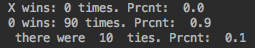
\includegraphics [scale=0.7]{QTable_vs_Minimax_untrained.png}
\end{flushleft}

Po przeuczeniu algorytmu na 20 000 grach z graczem losowym, zbiór $q_{s}$ ma 775 rekordów (tyle różnych stanów nasz agent napotkał), natomiast wyniki dla 100 gier teraz wyglądają już znacznie lepiej:
\begin{flushleft}
	\includegraphics [scale=0.7]{Qtable_vs_Rnd_trained.png}
\end{flushleft}
Z graczem losowym, wytrenowany agent przegrywa tylko w 3\%, ma 76\% wygranych i 21\% remisów. Grając z tak wytrenowanym agentem można odczuć, że gra całkiem dobrze, ale jeszcze czasami potrafi wykonać poważny błąd. \\

\begin{flushleft}
	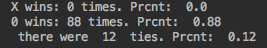
\includegraphics [scale=0.7]{QTable_vs_Minimax_trained.png}
\end{flushleft}
Nie ma natomiast prawie żadnej poprawy jeżeli chodzi o liczbę remisów (bo wygrać się nie da) z systemem grającym strategią minimax. Nasuwa się oczywiście pytanie, czy przetrenowanie algorytmu na grach z systemem grającym strategią minimax poprawiłoby tą statystykę?. Poniżej wyniki algorytmu po dodatkowym 10 000 grach z systemem grającym strategią minimax:

\begin{flushleft}
	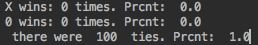
\includegraphics [scale=0.7]{QTable_vs_Minimax_trained_d.png}
\end{flushleft}
A więc trenowanie algorytmu na systemie grającym strategią minimax odniosło skutki.  Warto jeszcze sprawdzić, czy po tym trenowania algorytm nie odnotuje gorszych wyników grając z graczem losowym:
\begin{flushleft}
	\includegraphics [scale=0.7]{QTable_vs_Rnd_trained_d.png}
\end{flushleft}
Jak widać wyniki uległy nawet poprawie. Agent po dodatkowym trenowaniu wygrywa w 84\%, przegrywa w 2\% i w 14\% remisuje. Należy jednak zaznaczyć, że takie trenowanie algorytmu z systemem, który gra zgodnie ze strategią minimax, nie jest zupełnie zgodne z pierwotną ideą, żeby algorytm nauczył się grać w kółko i krzyżyk bez żadnych dodatkowych informacji, w tym bez możliwości uczenia się przez grę z optymalną strategią. \\

Na koniec dodam jeszcze, że po takim podwójnym trenowaniu, czysto subiektywne odczucie jest takie, że algorytm gra w sposób zbliżony do człowieka. Rzadko popełnia oczywiste błędy, a chwila nie uwagi kończy się zazwyczaj przegraną. 

 
\chapter{Sieć neuronowa grająca w kółko i krzyżyk }\label{r:Siec}

\section{Sieci neuronowe}
Metoda opisana w poprzednim rozdziale ma jedną zasadniczą wadę. Dla gier o znacznie większej liczbie możliwych kombinacji plansz, zbiory z wartościami $q_{s}$ stają się ogromne. O ile jeszcze samo zapisanie takiego zbioru, zważywszy na szybki rozwój elektronicznych nośników danych, mógłby być możliwy, to już przeszukiwanie przed każdym ruchem zbioru w celu wyłonienie tego, który maksymalizuje $q_{s}$ jest absolutnie nie wykonalne. Alternatywą do przechowywania wartości $q_{s}$ w tabeli lub pliku, może być wytrenowanie sieci neuronowej w taki sposób, żeby estymowała funkcję $s\rightarrow q_{s}$\\

Się neuronowa składa się z neuronów. Natomiast jeden neuron ma określoną liczbę danych wejściowych $n$, odpowiadającą tej ilości liczbę wag $w_{i}, 1 < i\leq n+1$, (o jeden więcej niż ilość danych wejściowych) przy czym oznaczymy $w_{n+1}=b$ , oraz zadaną funkcję aktywacji $f:\mathbf{R}\rightarrow\mathbf{R}$.  Załóżmy, że dane wejściowe to $x_{1}, x_{2},...,x_{n}$.  Neuron ,,bierze" sumę ważoną tych danych powiększoną o wyraz stały $w_{n+1}$ i zwraca wartość funkcji aktywacji z tej sumy :

%$$f(\sum_{i=1}^{n}w_{i}x_{i} +b)$$
\begin{flushleft}
	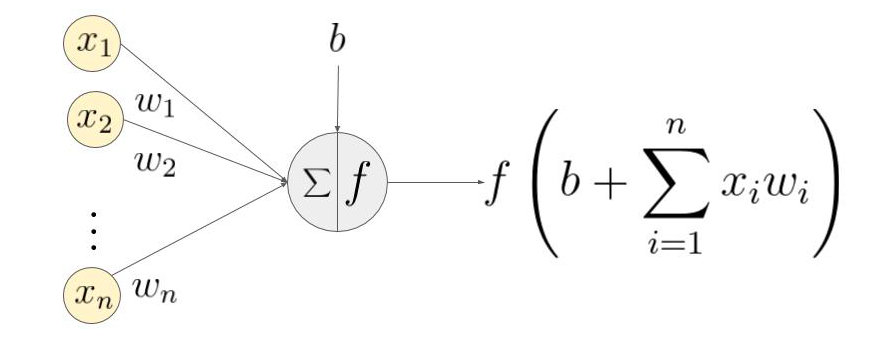
\includegraphics [scale=0.2]{neuron.png}
\end{flushleft}


Funkcje aktywacji może być w zasadzie dowolna. Ze względu łatwość ,,uczenia" sieci neuronowej, o czym za chwilę, warto stosować funkcje różniczkowalne (ewentualnie różniczkowalne poza kilkoma punktmai) i monotoniczne. Najczęściej stosuje się takie funkcje jak sigmoid, tanges hiporbeloczny, relu, czy softplus.  Poniżej definicja i wykres funkcji sigmoid - najbardziej klasycznego przykładu funkcji aktywacji.

$$sigmoid(x) = \frac{1}{1-e^{-x}}$$
\begin{flushleft}
	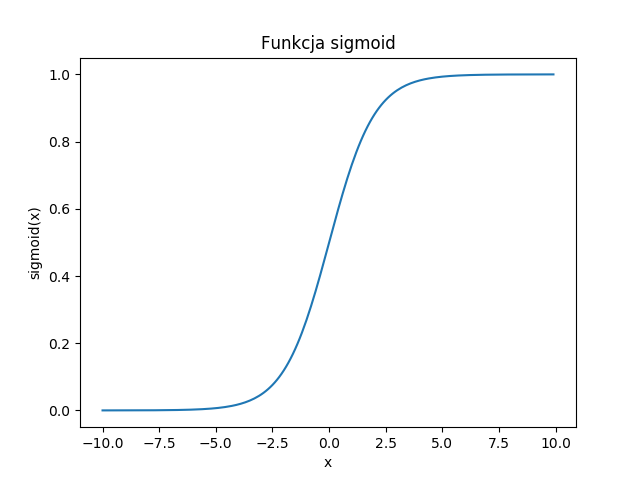
\includegraphics [scale=0.5]{sigmoid.png}
\end{flushleft}


Sieć neuronowa składa się, jak nazwa wskazuje z wielu neuronów, ułożonych w warstwy. Pierwsza warstwa, to warstwa wejściowa danych. Dane z wejściowe są przekazywane neuronom w w drugiej warstwie z neuronami. Każdy neuron ma swój zestaw wag, które służy do utworzenia kombinacji liniowej, z danych wejściowych, po czym neuron zwraca wartości funkcji aktywacji na tej kombinacji liniowej. Wartości zwracane przez neurony w drugiej warstwie są z kolei przekazywane do trzeciej warstwy z neuronami, tak jak dane wejściowe zostały przekazane do drugiej warstwy (pierwszej z neuronami).  Wartości obliczone na ostatniej warstwie z neuronami, to są wartości ostatecznie zwracane przez sieć. 

\begin{flushleft}
	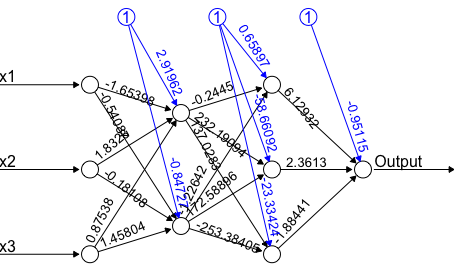
\includegraphics [scale=0.7]{nn_example.png}
\end{flushleft}

Rysunek powyżej przedstawia przykładową sieć, która ma trzy wartości wejściowe, a następnie warstwę 2 neuronów, warstwę 3 neuronów i ostatnią warstwę wyjściową składającą się z jednego neuronu. Wartości na strzałką pokazuję wartości wag neuronu, do którego prowadzi strzałka. Dodatkowo, na niebiesko zaznaczono wartości stałe ($b$) dla poszczególnych neuronów. Przy tworzeniu sieci neuronowej, ważne jest, żeby ilość wag dla każdego neuronu w k-tej warstwie, była równa ilości neuronów (lub danych wejściowych) w k-1-ej warstwie (plus dodatkowo wyraz stały). W przeciwnym razie nie uda się uwzględnić wszystkich wartości z k-1 warstwy w kombinacji liniowej.  \\
 
Podsumowując można powiedzieć, że siecią neuronową, o zadanej strukturze, jest funkcja $\mathbf{\mathcal{N}}$, której argumenty, to zbiór wartości wejściowych $x_{1},...,x_{n}$ oraz zbiór wszystkich wag $\mathbf{W}$ i zbiór wszystkich wyrazów stałych $\mathbf{b}$, która zwraca wektor wartości $y_{1},...,y_{m}$, którego wymiar jest równy ilości neuronów w ostatniej warstwie.

$$\mathcal{N}(x_{1},...,x_{n}, \mathbf{W}, \mathbf{b}) = (y_{1},...,y_{m})$$

Argumenty $\mathbf{W}$  i $\mathbf{b}$ będziemy traktować jak parametry funkcji $\mathbf{\mathcal{N}}$. Chcielibyśmy tak zmieniać te parametry, żeby sieć neuronowa $\mathbf{\mathcal{N}}$ przybliżała nam jakąś rzeczywistą, obserwowalną, ale nieznaną funkcję $\Phi$: 
$$ (x_{1},...,x_{n})\stackrel{\Phi}{\rightarrow}(y_{1},...,y_{m})$$

Skoro chcemy przybliżać funkcję $\Phi$ siecią neuronową $\mathbf{\mathcal{N}}$, to potrzebna jest jakaś miara skuteczności takiego przybliżenia.  Załóżmy, że mam k-elementowy zbiór danych $\mathbf{X}$ i dla każdego  $x_{1},...,x_{n}\in\mathbf{X}$ obserwujemy $\Phi(x_{1},...,x_{n})$ oraz $\mathbf{\mathcal{N}}(x_{1},...,x_{n}, \mathbf{W}, \mathbf{b})$. Jak w tym przypadku określić skuteczność przybliżania $\Phi$ za pomocą sieci $\mathbf{W}, \mathbf{b}$ na zbiorze $\mathbf{X}$? W literaturze można spotkać wiele metod, ale chyba najbardziej naturalną jest średnio kwadratowa funkcja straty (kosztu) , albo matematycznie norma $L_{2}$, którą zapiszemy jako funkcję parametrów $\mathbf{W}$ i $\mathbf{b}$.

$$C(\mathbf{W}, \mathbf{b}) = \frac{1}{2k}\sum_{(x_{1},...,x_{n})\in\mathbf{X}}{\norm{\Phi(x_{1},...x_{n}) - \mathbf{\mathcal{N}}(x_{1},...,x_{n}, \mathbf{W}, \mathbf{b} )}  } ^{2}$$

\section{Opis algorytmu}
W tej materii jeszcze niczego nie zrobiłem, ale będę walczył :-)

\chapter{Podsumowanie}

Tak jak zaznaczyłem we wprowadzeniu, tutaj opiszę - bardzo skrótowo - wrażenie z implementacji oraz podam jakieś informacje, który z algorytmów jest skuteczniejszy, szybszy i dlaczego. Na razie nic specjalnie mądrego nie przewiduję w tym rozdziale, ale wypadałoby, żeby jakieś podsumowanie było. Może po ukończeniu i przetestowaniu kodu, przyjdzie mi do głowy coś wartego napisania.

\appendix

\chapter{Kody}
Pytanie, czy warto tu umieszczać wszystkie, kody czy też nie ma sensu i może wystarczy link do gitHub'a.

\section{Klasa gry}

\begin{lstlisting}
        
        return line

\end{lstlisting}

\chapter{Aplikacja}

Tutaj zamieszczę krótki opis i "screen shot" z aplikacji do gry w kółko i krzyżyk.

\begin{thebibliography}{99}

\addcontentsline{toc}{chapter}{Bibliografia}

	\bibitem {nn} Michael Nielsen, \textit{Neural Networks and Deep Learning}, Determination Press, 2015

	\bibitem {itsl} James Gareth, \textit{Introduction to Statistical Learning}, Springer, 2013
	
	\bibitem {RL} Richard S. Sutton and Andrew G. Barto, \textit{Reinforcement Learning: An Introduction},  MIT Press, Cambridge, MA, 2018
	
	\bibitem {MIT_AI} Prof. Patrick Henry Winston, \textit{MIT course number 6.043, Artifical Inteligence}, https://ocw.mit.edu/courses/electrical-engineering-and-computer-science/6-034-artificial-intelligence-fall-2010/index.htm
	
	\bibitem{Game} Matthew O. Jackson , \texit{A Brief Introduction to the Basics of Game Theory},\linebreak https://www.ethz.ch/content/dam/ethz/special-interest/gess/chair-of-sociology-dam/documents/education/spieltheorie/literatur/Einführung/Jackson\linebreak\%20Basics\%20of\%20Game\%20Theory\%20SSRN-id1968579.pdf

\end{thebibliography}

\end{document}


%%% Local Variables:
%%% mode: latex
%%% TeX-master: t
%%% coding: latin-2
%%% End:
